\documentclass[pdf, azure]{prosper}
\usepackage[utf8]{inputenc}
%\usepackage[latin1]{inputenc}
\usepackage[spanish]{babel}
\usepackage{amsmath}
\usepackage{anysize}
\usepackage{graphics}
\title{Curso de Física Computacional}
\subtitle{Diferenciación numérica}
\author{M. en C. Gustavo Contreras Mayén}
\email{curso.fisica.comp@gmail.com}
\ptsize{10}
\begin{document}
\maketitle
\begin{slide}{Diferenciación numérica}
Consideremos una función $f(x)$, nuestro interés será evaluar la primera derivada de esta función en el punto $x = x_{0}$
\\
Si conocemos los valores de $f$ en $x_{0}-h$, $x_{0}+h$, donde $h$ es el tamaño del intervalo entre dos puntos consecutivos en el eje $x$, entonces podremos aproximar $f'(x_{0})$ mediante un gradiente de interpolación lineal A, B o C.
\end{slide}
\begin{slide}{Diferencias hacia adelante}
Aproximación por A
\[ f'(x_{0})=  \dfrac{f(a)-f(b)}{h} \]
\begin{center}
	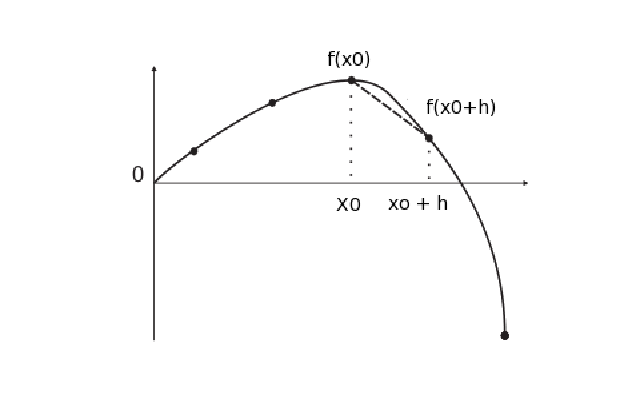
\includegraphics[scale=0.35]{Dif_A.ps} 
\end{center}
\end{slide}
\begin{slide}{Diferencias hacia atrás}
Aproximación por B
\[ f'(x_{0}) = \dfrac{f(x_{0})-f(x_{0}-h)}{h} \]
\end{slide}
\begin{slide}{Diferencias centrales}
Aproximación por C
\[ f'(x_{0}) = \dfrac{f(x_{0}-h)-f(x_{0}+h)}{h} \]
\begin{center}
	\includegraphics[scale=0.35]{Dif_C.ps} 
\end{center}
\end{slide}
\begin{slide}{Solución por Serie de Taylor}
Cuando tenemos una función que se representa por puntos discretos, la aproximación que podemos hacer, es mediante una interpolación.
\\
De manera análoga al caso de la integración, existen fórmulas de diferenciación numérica si derivamos las fórmulas de interpolación.
\end{slide}
\begin{slide}{Continuamos}
Para una derivada de orden $p$, se requiren de al menos $p+1$ datos, para obtener una aproximación por diferencias.
\bigskip
Veamos el caso para $f'_{i} = f'(x_{i})$ usando $f_{i}=f(x_{i})$ y $f_{i+1}=f(x_{i+1})$. Los valores de $f$ en todos los puntos distintos de $x_{i}$ se desarrollan en una serie de Taylor.
\end{slide}
\begin{slide}{La serie}
Haciendo el desarrollo de Taylor de $f_{i+1}$ alrededor de $x_{i}$, es:
\[ f_{i+1} = f_{i} + hf'_{i} + \dfrac{h^{2}}{2} f''_{i} + \dfrac{h^{3}}{6} f'''_{i} + \dfrac{h^{4}}{24} f^{iv}_{i} + \cdots \]
\end{slide}
\begin{slide}{Serie truncada}
Al truncar luego del primer término, la ecuación anterior es la aproximación por diferencias hacia adelante:
%\begin{eqnarray*}
%f'_{i} & = & \dfrac{f_{i+1} - f_{i}}{h} + O(h)} \nonumber \\
%O(h) & = & -\dfrac{h}{2} f''_{i} 
%\end{eqnarray*}
El término $O(h)$ indica que el error es aproximadamente proporcional al intervalo $h$ de la retícula. El error también es proporcional a la segunda derivada $f''$.
\end{slide}
\begin{slide}{ \ptsize{12} Aproximación por diferencias hacia atrás}
La aproximación por diferencias hacia atrás de la primera derivada, utilizando $f_{i-1}$ y $f_{i}$, se estima de la misma forma que la anterior. El desarrollo de Taylor de $f_{i-1}$ es:
\[ f_{i-1}= f_{i}-hf'_{i}+ \dfrac{h^{2}}{2} f''_{i} - \dfrac{h^{3}}{6} f'''_{i} + \dfrac{h^{4}}{24} f^{iv}_{i} -\cdots \]
\end{slide}
\begin{slide}{Aproximación}
Despejando $f'_{i}$, obtenemos la aproximación por diferencias hacia atrás:
\begin{eqnarray*}
f^{'}_{i}  =  \dfrac{f_{i}-f_{i-1}}{h} + O(h)} \\
O(h)  =  \dfrac{h}{2} f^{''}_{i}
\end{eqnarray*}
\end{slide}
\end{document}